\documentclass{article}
\usepackage[utf8]{inputenc}
\usepackage{amsmath}
\usepackage{graphicx}
\usepackage{hyperref}
\usepackage{geometry}
\geometry{a4paper, margin=1in}

\title{Análisis Comparativo de Métodos de Optimización para una Función No Convexa}
\author{Kevin Alejandro Torres Perera \\ Grupo: C311}
\date{\today}

\begin{document}

\maketitle

\href{https://github.com/KevinTorres01/OptimProject}{Enlace al proyecto en GitHub}

\begin{figure}[h!]
    \centering
    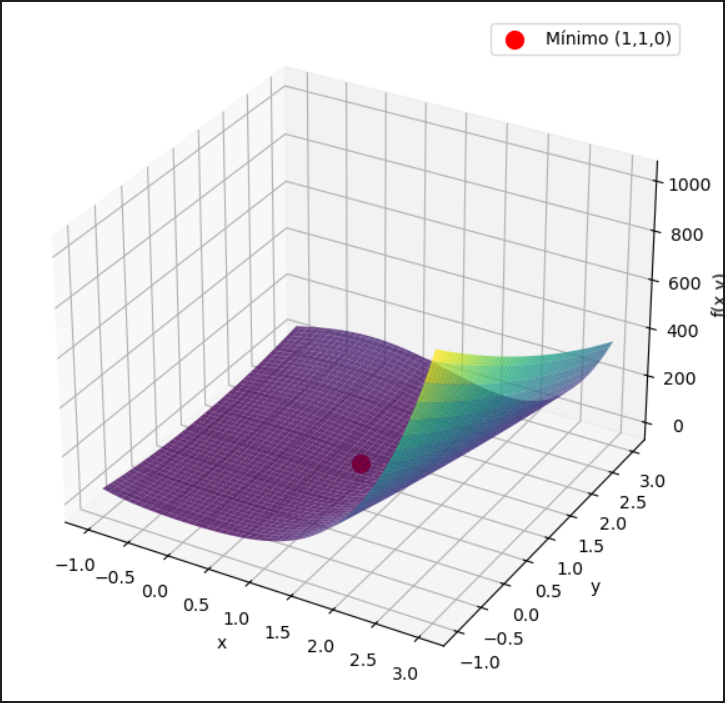
\includegraphics[width=0.8\textwidth]{3DGraphication.png}
    \caption{Visualización 3D de la función objetivo.}
    \label{fig:3dgraph}
\end{figure}

Este informe presenta un análisis teórico y experimental del problema de minimización para la función no convexa $f(x,y) = 10(y - x^2)^2 + \frac{(x-1)^2}{2} + (y-1)^2$. El estudio tiene como objetivo caracterizar matemáticamente la función, determinar su mínimo teórico y, fundamentalmente, evaluar y comparar el rendimiento de dos algoritmos de optimización: el método de Newton con Gradiente Conjugado (Newton-CG) y el método quasi-Newton BFGS.

\section{Análisis del Modelo}

El problema consiste en la minimización sin restricciones de una función definida en $\mathbb{R}^2$. A continuación, se analiza la existencia de solución y la convexidad del modelo.

\subsection{Existencia de Solución}
La función objetivo es continua en todo su dominio. Además, es una función coercitiva, lo que significa que $f(x,y) \to \infty$ cuando la norma del vector $(x,y)$ tiende a infinito. Esto se debe a los términos cuadráticos dominantes. Según el Teorema de Weierstrass, toda función continua y coercitiva sobre $\mathbb{R}^n$ alcanza un mínimo global. Por lo tanto, la existencia de al menos una solución para el problema de minimización está garantizada.

\subsection{Convexidad}
Como se detallará en el análisis de la matriz Hessiana, la función no es convexa globalmente. La falta de convexidad implica que los algoritmos de optimización podrían, en teoría, converger a mínimos locales en lugar del mínimo global. Sin embargo, para este problema particular, se demostrará que existe un único punto estacionario que corresponde al mínimo global, simplificando el desafío que la no convexidad podría presentar.

\section{Caracterización de la Función Objetivo}

La función objetivo a minimizar está definida en el dominio $\mathbb{R}^2$, ya que las operaciones que la componen —polinomios, sumas y productos— son válidas para cualquier par de números reales. Un análisis de sus términos revela que la función es no negativa en todo su dominio, dado que cada componente es un término cuadrático multiplicado por una constante positiva. La función alcanza su valor mínimo de cero si y solo si todos sus términos son simultáneamente nulos, lo cual ocurre únicamente en el punto $(1, 1)$. En cualquier otro punto, la función es estrictamente positiva.

La función es una composición de polinomios y combinaciones lineales, por lo que es continua en todo su dominio. Además, al ser un polinomio en las variables $x$ e $y$, todas sus derivadas parciales de cualquier orden existen y son continuas. Esto implica que la función es infinitamente diferenciable, o suave ($C^\infty$), lo que garantiza las condiciones de regularidad necesarias para aplicar métodos de optimización basados en el cálculo diferencial.

\section{Gradiente y Matriz Hessiana}

El gradiente de la función, $\nabla f(x,y)$, que indica la dirección de máximo crecimiento, se obtiene calculando las derivadas parciales con respecto a $x$ e $y$. El resultado es el siguiente vector:

\[
\nabla f(x,y) = \begin{bmatrix} 40x^3 - 40xy + x - 1 \\ 22y - 20x^2 - 2 \end{bmatrix}
\]

La matriz Hessiana, $H(x,y)$, que describe la curvatura local de la función, se compone de las segundas derivadas parciales:

\[
H(x,y) = \begin{bmatrix} 120x^2 - 40y + 1 & -40x \\ -40x & 22 \end{bmatrix}
\]

El análisis de la Hessiana es crucial para entender la convexidad de la función. Una función es estrictamente convexa si su matriz Hessiana es definida positiva en todo su dominio. Sin embargo, en este caso, se puede demostrar que la función no es convexa globalmente. Por ejemplo, en el punto $(0, 1)$, el primer elemento de la diagonal de la Hessiana es negativo ($H_{11} = -39$) y su determinante también es negativo, lo que confirma que la matriz no es definida positiva. Esta no convexidad puede presentar desafíos para los algoritmos de optimización, aunque no impide la existencia de un mínimo global único.

\section{Determinación del Mínimo Teórico}

Para encontrar los candidatos a óptimos en un problema sin restricciones, se buscan los puntos estacionarios, es decir, aquellos donde el gradiente se anula. Al resolver el sistema de ecuaciones $\nabla f(x,y) = \mathbf{0}$, se encuentra que la función posee un único punto estacionario en $(1, 1)$.

Para clasificar este punto, se evalúa la matriz Hessiana en $(1, 1)$, resultando en:

\[
H(1,1) = \begin{bmatrix} 81 & -40 \\ -40 & 22 \end{bmatrix}
\]

Esta matriz es definida positiva, ya que su primer elemento diagonal es positivo (81) y su determinante también lo es (182). Según el criterio de la segunda derivada, esto confirma que el punto $(1, 1)$ es un mínimo local estricto. Dado que ya se ha establecido que $f(1,1)=0$ es el valor más bajo que la función puede tomar en todo su dominio, se concluye que $(1, 1)$ es también el mínimo global único.

\section{Descripción de los Algoritmos Evaluados}

\subsection{Método de Newton-CG}

El método de Newton con Gradiente Conjugado (Newton-CG) es una variante del método de Newton clásico, optimizado para problemas a gran escala. En lugar de calcular y almacenar la inversa de la matriz Hessiana, utiliza el método del gradiente conjugado para resolver de forma iterativa el sistema lineal asociado en cada paso. Este enfoque le permite aprovechar la información de la curvatura de segundo orden para lograr una convergencia teórica cuadrática cerca del óptimo, lo que idealmente se traduce en un menor número de iteraciones.

\subsection{Método Quasi-Newton BFGS}

El método BFGS (Broyden-Fletcher-Goldfarb-Shanno) es uno de los algoritmos quasi-Newton más eficaces. Su principal característica es que no requiere el cálculo explícito de la matriz Hessiana. En su lugar, construye y actualiza una aproximación de la Hessiana inversa en cada iteración, utilizando únicamente la información del gradiente. Este enfoque le permite alcanzar una convergencia superlineal, que, aunque teóricamente más lenta que la de Newton, resulta computacionalmente más ligera por iteración y, a menudo, más robusta en la práctica, especialmente en funciones no convexas.

Ambos algoritmos fueron implementados en este proyecto utilizando la función \texttt{scipy.optimize.minimize} de la biblioteca SciPy en Python. Esta función proporciona una interfaz unificada para una amplia gama de algoritmos de optimización. Para invocar los métodos específicos, se pasó el nombre del algoritmo ('Newton-CG' o 'BFGS') en el parámetro \texttt{method}. Puede encontrar más detalles en la \href{https://docs.scipy.org/doc/scipy/reference/generated/scipy.optimize.minimize.html}{documentación oficial de SciPy}.

\section{Análisis de Resultados Experimentales}

Para evaluar el rendimiento práctico de ambos algoritmos, se ejecutó un conjunto de 34 experimentos con puntos iniciales distribuidos en diferentes zonas del dominio y con distintas tolerancias. El análisis de los resultados almacenados revela patrones de comportamiento claros y consistentes.

La conclusión más destacada es la superioridad en robustez del método BFGS. A lo largo de todos los experimentos, BFGS convergió exitosamente al mínimo global, independientemente del punto de partida. En contraste, el método Newton-CG mostró ser frágil, fallando en varias configuraciones, especialmente aquellas con puntos iniciales muy alejados del óptimo. Los resultados de \texttt{results\_exp1.json} y \texttt{results\_exp2.json} muestran advertencias para Newton-CG como \texttt{Warning: CG iterations didn't converge. The Hessian is not positive definite}. Esto confirma empíricamente que la no convexidad de la función en ciertas regiones impide que el subproblema del gradiente conjugado se resuelva adecuadamente, llevando al fallo del algoritmo.

En términos de eficiencia, aunque la teoría sugiere que Newton-CG podría requerir menos iteraciones, en la práctica su mayor costo computacional por iteración lo penaliza. Los datos experimentales muestran que, en la mayoría de los escenarios, BFGS alcanzó la solución en un tiempo de ejecución total menor. Incluso en casos donde el número de iteraciones fue similar, la ligereza de los cálculos de BFGS le otorgó una ventaja decisiva en velocidad.

En cuanto a la precisión, ambos métodos fueron capaces de localizar el mínimo con una exactitud muy alta, alcanzando valores de la función objetivo extremadamente cercanos a cero. Sin embargo, la fiabilidad de BFGS para lograr esta precisión en el 100\% de los casos, en contraposición a los fallos de Newton-CG, lo consolida como el método más predecible y seguro para este problema.

\section{Conclusiones Finales}

El análisis comparativo entre Newton-CG y BFGS para la minimización de esta función no convexa arroja conclusiones de gran relevancia práctica.

Primero, la robustez es un factor crítico. El método BFGS demostró ser significativamente más robusto, garantizando la convergencia desde todos los puntos iniciales probados. La dependencia de Newton-CG de una matriz Hessiana definida positiva lo vuelve vulnerable en paisajes de optimización complejos.

Segundo, la eficiencia teórica no siempre se traduce en un mejor rendimiento práctico. El menor costo por iteración de BFGS resultó en una mayor eficiencia global, superando a Newton-CG en tiempo de ejecución en la mayoría de los experimentos.

En definitiva, para el problema estudiado, el algoritmo BFGS ofrece el mejor compromiso entre velocidad, precisión y, fundamentalmente, robustez. Su enfoque de aproximar la información de segundo orden en lugar de calcularla directamente le confiere la flexibilidad necesaria para navegar por el dominio no convexo de manera eficaz y fiable. Por lo tanto, se concluye que BFGS es la elección pragmática y superior para esta clase de problemas de optimización.

\end{document}
